\documentclass[draft=false]{assignment}

\usepackage{float}
% \usepackage{tikz}
\usepackage{circuitikz}
\usepackage{adjustbox}
\usepackage{titlesec}
\usepackage{soul}
\usepackage{csvsimple}

\usepackage{graphicx}
\usepackage{subcaption}
\usepackage{pgfgantt}
\usetikzlibrary{shapes, arrows}

\usetikzlibrary{calc,patterns,angles,quotes}
\setlength{\parindent}{0pt}

\hypersetup{
pdftitle={Lab - Mechatronics},
pdfsubject={Report for the MagLev laboratory experience},
pdfauthor={Tommaso Bocchietti, Daniele Cianca, Sara Orazzo},
pdfkeywords={Politecnico di Milano, Mechatronics, Magnetic Levitation System}
}

\makenoidxglossaries
\newacronym{mls}{MLS}{Magnetic Levitation System}
\newacronym{siso}{SISO}{Single Input Single Output}
\newacronym{miso}{MISO}{Multiple Input Single Output}
\newacronym{mimo}{MIMO}{Multiple Input Multiple Output}
\newacronym{pid}{PID}{Proportional Integral Derivative}
\newacronym{mpc}{MPC}{Model Predictive Control}
\newacronym{lqr}{LQR}{Linear Quadratic Regulator}

\begin{document}

\title{Lab - Mechatronics \\ Modelling and control of a Magnetic Levitation System}
\author{Tommaso Bocchietti 10740309 \\ Daniele Cianca 10764733 \\ Sara Orazzo 10995845}
\date{A.Y. 2024/25}

\maketitle

\begin{figure}[H]
    \centering
    
\includegraphics[width=0.7\textwidth]{./pdf/Polimi_logo_coverpage.pdf}
    \label{fig:Polimi_logo}
\end{figure}

\clearpage
\tableofcontents
\listoffigures
\listoftables
\lstlistoflistings
% \printnoidxglossaries

\clearpage
\begin{frame}{Introduction}

    \hl{Do we want to explain the MagLev?}

    Composed of:

    \begin{itemize}
        \item The ball
        \item The electromagnet
        \item The controll unit (Arduino)
    \end{itemize}

    Etc..

\end{frame}

\clearpage
\section{Magnetic Levitation System}
\label{sec:magnetic_levitation_system}

As stated in the introduction, the system under study is the \acrfull{mls} provided by \texttt{Inteco} (producer website: \url{https://www.inteco.com.pl/products/magnetic-levitation-systems/}).
In Figure \ref{fig:MLS} the system used in this work is shown.

\begin{figure}[H]
    \centering
    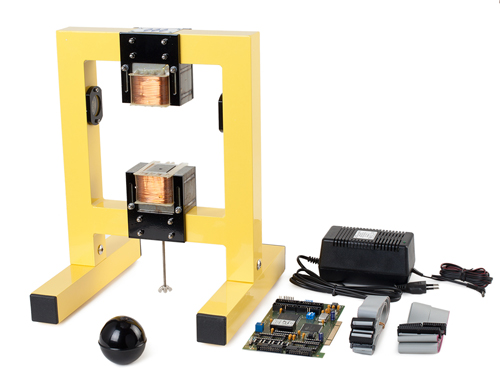
\includegraphics[width=0.7\textwidth]{./img/maglev_and_components.jpg}
    \caption{\acrlong{mls}}
    \label{fig:MLS}
\end{figure}

As it can be seen quite clearly, the system is composed of a simple mechanical structure that is used to support two electromagnets and an optical infrared sensor.
Along with the mechanical structure, a ferromagnetic ball and a control unit are present.

At its core principle, the system uses the interaction between the magnetic field generated by the electromagnets and the ferromagnetic ball to keep the ball in a desired position.
The optical sensor is used to measure the position of the ball and provide feedback to the control unit that, in turn, adjusts the voltage applied to (and indeed the current flowing through) the electromagnets to keep the ball in a desired position.
In Figure \ref{fig:MLS_general_scheme} a schematic representation of the upper half of the system is shown.

\begin{figure}[H]
    \centering
    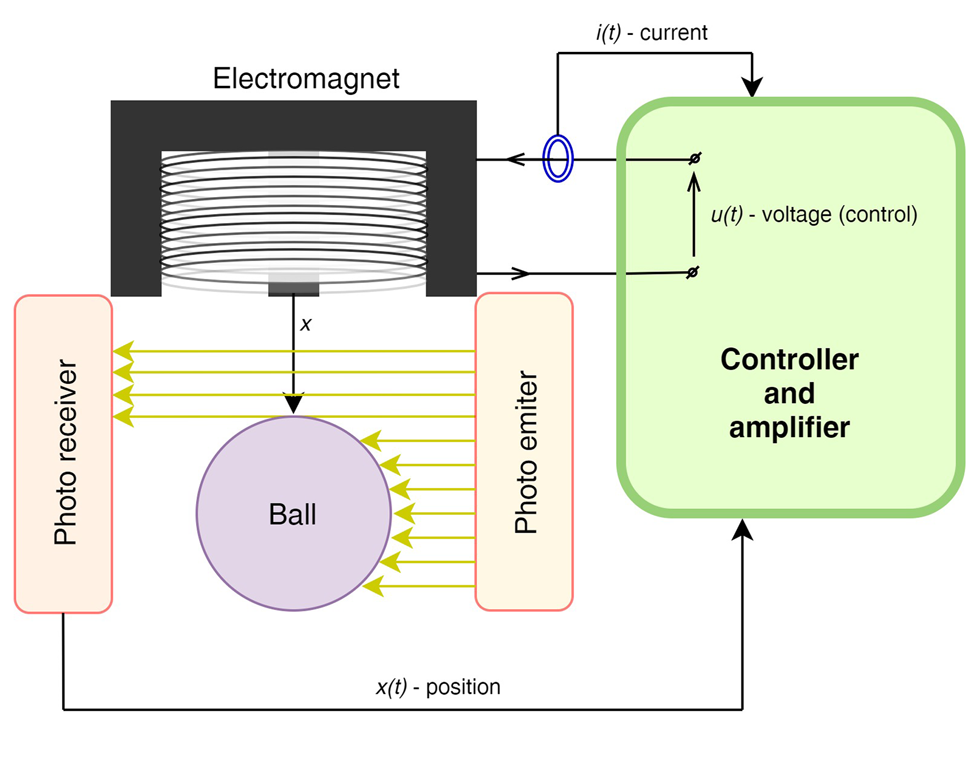
\includegraphics[width=0.9\textwidth]{./img/maglev_general_scheme.png}
    \caption{Schematic representation of the upper half of the \acrshort{mls} system.}
    \label{fig:MLS_general_scheme}
\end{figure}

\paragraph{Real world application}

Despite the fact that our system is a simplified use case, the magnetic levitation principle is used in many real-world applications.

One of the most common applications is the magnetic levitation trains, also known as `MagLev' trains.
These trains use the magnetic levitation principle to lift the train off the tracks and propel it forward using the magnetic field generated by the tracks.
The main advantage of this technology is the absence of friction between the train and the tracks, which allows the train to reach higher speeds and reduce the noise characteristic of the traditional trains.
Some of the fastest (operating) trains in the world are MagLev trains, with the Shanghai MagLev train being the fastest, reaching a top speed of $623 km/h$ \cite{WikiSCMaglev}.

Another application of the magnetic levitation principle is the magnetic bearings.
These bearings use the magnetic field generated by electromagnets to levitate a rotor and keep it in a desired position.
The main advantage of this technology is the absence of mechanical contact between the rotor and the stator, which allows the rotor to reach higher speeds and reduce the wear of the components.

\clearpage
\section{Controller Design}
\label{sec:controller_design}

Based on the MLS2EM datasheet/manual, some suggestions are (page 5):

\begin{itemize}
    \item SISO, MISO, BIBO controllers design
    \item Intelligent/Adaptive Control
    \item Frequency analysis
    \item Nonlinear control
    \item Hardware-in-the-Loop
    \item Real-Time control
    \item Closed Loop PID Control
\end{itemize}

From `Gruppo 1 MagLev', the following controllers are suggested:

\begin{itemize}
    \item prova\_2PID\_EKF.slx
    \item prova\_3\_anelli\_stabilizzante.slx
    \item prova\_3\_anelli\_stabilizzante\_v2.slx
    \item prova\_backstepping.slx
    \item prova\_cascata.slx
    \item prova\_funzionante\_filtro.slx
    \item prova\_funzionante\_finale\_PID2.slx
    \item prova\_funzionante\_LQR.slx
    \item prova\_funzionante\_LQR\_EKF.slx
    \item prova\_funzionante\_LQR\_int.slx
    \item prova\_funzionante\_LQR\_in\_PIDt.slx
    \item prova\_funzionante\_LQR\_noint.slx
    \item prova\_funzionante\_obs.slx
    \item prova\_funzionante\_PP.slx
    \item prova\_funzionante\_PP\_2EM.slx
    \item prova\_funzionante\_PP\_EKF.slx
    \item prova\_funzionante\_PP\_int.slx
    \item prova\_funzionante\_PP\_int\_obs.slx
    \item prova\_funzionante\_PP\_KF.slx
    \item prova\_funzionante\_PP\_OBS.slx
    \item prova\_funzionante\_PP\_OBS2.slx
    \item prova\_funzionante\_sinusoidi.slx
    \item prova\_pid\_variabile.slx
\end{itemize}

That should correspond to the following controllers:

\begin{itemize}
    \item Simple PID
    \item Variable PID (coefficients computed on the fly)
    \item Linear Quadratic Regulator (LQR)
    \item Kalman Filter (KF)
    \item Extended Kalman Filter (EKF)
    \item Observers
    \item Backstepping (?)
    \item Cascaded controllers (outer: voltage, inner: current)
\end{itemize}

\subsection{PD Controller}
\label{sec:pd}

The Proportional-Derivative (PD) controller is a simple controller that uses the error signal and its derivative to compute the control signal.
Its derived from the Proportional-Integral-Derivative (PID) controller, which is one of the most common controllers used in industry, with a control signal given by:

\begin{equation}
    u(t) = K_p e(t) + K_i \int_{0}^{t} e(\tau)dt + K_d \frac{de(t)}{dt} = K_p \left(e(t) + \frac{1}{T_i} \int_{0}^{t} e(\tau)dt + T_d \frac{de(t)}{dt}\right)
\end{equation}

Where $K_p$, $K_i$ and $K_d$ are the proportional, integral and derivative gains, respectively, and $T_i$ and $T_d$ are the integral and derivative time constants, respectively.

Given that our system doesn't have a friction term at steady state condition, the integral action that ensures zero steady-state error is not necessary and can be omitted (i.e. $K_i = 0$).

In order to controll the \acrshort{mls} system, we need to linearize the system around a desired operating point, and tune the controller gains accordingly.


% \input{src/03.2 - pd_online_coefficients.tex}


\clearpage
\section{Controllers Comparison}
\label{sec:controllers_comparison}

\clearpage
\section{Conclusions}
\label{sec:conclusions}

\clearpage
\bibliographystyle{plain}
\bibliography{bibliography}

% \clearpage
% \appendix


\end{document}
